\documentclass{standalone}
\usepackage{tikz}
\begin{document}
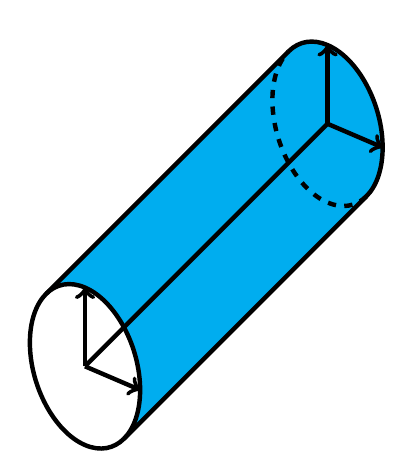
\begin{tikzpicture}
\begin{scope}[x={(.7cm,-.3cm)}]
\path (1,0,0);
\pgfgetlastxy{\cylxx}{\cylxy}
\path (0,1,0);
\pgfgetlastxy{\cylyx}{\cylyy}
\path (0,0,1);
\pgfgetlastxy{\cylzx}{\cylzy}
\pgfmathsetmacro{\cylt}{(\cylzy * \cylyx - \cylzx * \cylyy)/ (\cylzy * \cylxx - \cylzx * \cylxy)}
\pgfmathsetmacro{\ang}{atan(\cylt)}
\pgfmathsetmacro{\ct}{1/sqrt(1 + (\cylt)^2)}
\pgfmathsetmacro{\st}{\cylt * \ct}
\fill[cyan] (\ct,\st,0) -- ++(0,0,-8) arc[start angle=\ang,delta angle=180,radius=1] -- ++(0,0,8) arc[start angle=\ang+180,delta angle=-180,radius=1];
\begin{scope}[every path/.style={ultra thick}]
\draw (0,0,0) circle[radius=1];
\draw[->] (0,0,0) -- (1,0,0);
\draw[->] (0,0,0) -- (0,1,0);
\draw[->] (0,0,-8) -- (0,1,-8);
\draw[->] (0,0,-8) -- (1,0,-8);
\draw[-] (0,0,0) -- (0,0,-8);
\draw (\ct,\st,0) -- ++(0,0,-8);
\draw (-\ct,-\st,0) -- ++(0,0,-8);
\draw (\ct,\st,-8) arc[start angle=\ang,delta angle=180,radius=1];
\draw[dashed] (\ct,\st,-8) arc[start angle=\ang,delta angle=-180,radius=1];
\end{scope}
\end{scope}
\end{tikzpicture}
%source: http://tex.stackexchange.com/questions/31548/drawing-simple-3d-cylinders-in-tikz
\end{document}
